\documentclass[]{report}
\usepackage[utf8]{inputenc}
\usepackage{setspace}
\usepackage{footmisc}
\usepackage{marginnote}
\usepackage{sidenotes}
	\renewcommand{\thesidenote}{\number{\setcounter{secnumdepth}{0}}}
	\newcommand{\sidenotefont}{\footnotesize{6}}
	\newcommand{\sidenotecolor}{blue}	
	\newcommand{\sidenotespace}{\singlespacing}
\usepackage[brazilian]{babel}
\usepackage{graphicx} %imagens
\usepackage[hycap]{caption} %legenda
\usepackage[colorlinks=true, allcolors=blue]{hyperref}
\usepackage{titlesec}
\usepackage{ulem}
\usepackage{enumitem}
	\setlist[enumerate]{itemsep=1ex,parsep=1ex}
\usepackage{geometry}
\geometry{
  a4paper,
  twoside,
  inner=2cm, % Margem interna (vinculada)
  outer=5cm, % Margem externa (aberta)
  top=2cm,
  bottom=2cm,
}

\singlespacing

% Title Page
\title{\textbf{Morphoadæquabilitas}: Um Conjunto de Diretrizes para o Projeto de Traçados Urbanos Morfologicamente Adequados ao Contexto como alternativa ao \textit{Modus Faciendi} atual}
\author{Higor Ribeiro da Costa}



\begin{document}
\maketitle

\tableofcontents

\begin{abstract}
\end{abstract}

	%\geometry{top=3cm, bottom=2cm, left=2cm, right=5cm}
	\chapter*{Introdução}
	\addcontentsline{toc}{chapter}{Introdução}
	\onehalfspacing

	No fim de minha dissertação, cheguei à conclusão de que é possível projetar traçados urbanos morfologicamente adequados ao contexto. E explico o que quero dizer com isso. `Contexto' aqui é o conjunto de estruturas naturais e antrópicas de uma área com suas respectivas características, suas variáveis. `Morfologicamente adequado' quer dizer aquilo que já é, desde sua concepção, coerente com o formato das estruturas do contexto dado pela realidade. E traçado urbano é a marca das estruturas urbanas que o homem desenvolve.
	
	No caso das estruturas naturais, o que tomo por mais importante é a orografia, a terra com a sua forma, que é sobre onde se assentam as estruturas que o homem desenvolve, seguida pela hidrografia. Uma área pode ser mais íngreme ou suave, mais ou menos extensa, e seu relevo possui uma hierarquia latente, que pode ser destrinchada por meio de cumeadas, pontos de distribuição, assim como por talvegues e pontos de encontro. E, no caso das estruturas antrópicas, temos parcelamentos rurais precedentes, franjas urbanas com loteamentos, e diretrizes viárias. Com isso, temos ruas e avenidas, lotes urbanos e glebas rurais com seus limites. Cada uma dessas estruturas naturais e antrópicas desenvolve uma relação de interdependência, existencial – pois algumas não podem existir sem outras – e morfológica, por meio de seus formatos poligonais e consequentes angulações – bidimensional ou tridimensionalmente. 
	
	Ou seja, quando digo que um traçado urbano deve ser `morfologicamente adequado ao contexto', quero implicar que cada um de seus elementos (sobretudo ruas, praças, demais espaços abertos, e os lotes e quarteirões que derivam de sua disposição) deve, na máxima medida possível, seguir, primeiro, os formatos dados pela estruturação natural, e segundo, os formatos dados pelos elementos da estruturação antrópica. E isso se opõe ao \textit{laissez-faire} dos traçados `hilemórficos' concebidos \textit{a priori} e só depois `adaptados' à realidade, que se impõe forçosamente ao projetista contrariado. Um traçado `adequado' é diferente de um traçado `adaptado'. É a morfogênese planejada contraposta ao hilemorfismo autômato.\footnote[1]{\textit{``The hylomorphic model has dominated the relationship between matter and form within Western culture. The term ‘hylomorph’ indicates what is needed to design, for example, a table. It derives from \textnormal{hyle}, meaning wood, and morph, meaning form. So when we design a table by means of the hylomorphic model, we take a form \textnormal{(morph)} – the image of the table we would like to design – and press it into the wood \textnormal{(hyle)} – the material by which the image should come alive. The effect is a copy, a representation of what we imagined a table should look like."} (Trummer, 2009).}
	
	\begin{center}
		. . . . .
	\end{center}

	%É possível projetar traçados urbanos morfologicamente adequados ao contexto. Como assim? Na presente tese, dirijo-me aos profissionais, pesquisadores, docentes e estudantes que terão de desenhar ruas. Ruas dão acesso a edificações. Edificações inseridas em lotes. Lotes que formam quarteirões, que formam bairros, que formam cidades: organismos urbanos cuja `marca' no solo pode ser chamada de `traçado'. Traçado esse que é colocado de maneira mais ou menos consoante a um contexto, \textit{i. e.,} um conjunto de estruturas naturais subjacentes – colinas, planícies com suas topografias – e, eventualmente, estruturas antrópicas pré-existentes – como parcelamentos rurais, traçados e diretrizs viárias. Voltando: é possível projetar, conceber 

	%É possível projetar traçados urbanos morfologicamente adequados ao contexto. Não `adaptados' \textit{a posteriori,} mas `adequados' desde sua gênese: desenhados, concebidos \textit{a priori} precisa e especificamente para um contexto, não se encaixando em nenhum outro lugar. E acrescento: isso é possível por meio de um conjunto de diretrizes de projeto. 
	
	Durante aquela pesquisa, da qual a presente tese não é senão a continuação, desenvolvi o conceito de `\textit{rendimento} urbano' – que afirma que deve existir uma ``coerência intrínseca entre o traçado da forma urbana e o contexto natural" (Costa e Rego, 2019, p. 7); e projetei um traçado urbano hipotético sobre uma área urbana consolidada, comparando-o com o traçado existente e com a legislação local em vigor. Com isso, verifiquei ser possível projetar traçados urbanos `de qualidade' (Costa, 2020, p. 106). Traçados com bom \textit{rendimento} urbano. %hipótese é quando temos variáveis mensuráveis; porém, quando temos variáveis qualitativas ou de `constructos', o que temos é uma `proposição'.
	
	%Questão/variáveis: uma das variáveis dos traçados: angulação (bidimensional (mapa) e tridimensional (com curvas de nível e perfis de elevação))

	%%Questão principal → Hipótese principal → Questão secundária → hip. sec.
	%% Verificar hipótese com variáveis que estão presentes nas diretrizes de projeto.
	%% Melhorar hipótese ou gerar hipóteses subordinadas. 
	%% Explicar variáveis já no início (variáveis que PODEM vir da teoria, eg., teoria Caniggiana)

	%%Ou Hipótese vinculada a uma teoria (Caniggia → Hipótese) → pergunta derivada à hipótese.

	O que fiz na dissertação foi uma simulação baseada na síntese de um novo conceito (o \textit{rendimento} urbano) e em um estudo de caso (a partir do qual foram extraídos parâmetros para a avaliação desse conceito). Eu queria mostrar que um traçado urbano adequado ao sítio tinha lugar no mundo contemporâneo das cidades planejadas \textit{a priori}, posto que, hoje, um processo de desenvolvimento gradual da estrutura urbana, do traçado urbano, parece já não ter lugar – pois o \textit{status quo}, hoje, é o da morfogênese substituída pelo hilemorfismo. 
	
	Outrora, as ruas não eram senão a afirmação de percursos pré-existentes, sulcados ao longo do tempo no relevo do território por inúmeras gerações que nos precederam – segundo Caniggia e Maffei (2008), remontando ao período neolítico. Esses percursos, primitivamente utilizados apenas como rotas de passagem, passaram a ser a estrutura de acesso a áreas inicialmente de caça e coleta, posteriormente de cultivo, até chegar à sua partição em propriedades. E, nos locais mais propícios, tais percursos tiveram seus formatos consolidados, consagrados na matéria, por meio das fachadas as edificações que os margeavam. Era a formação do que, no universo lusófono, chamamos de ``rua", com a série de edificações a ela rentes.
	
	Observando esse processo, não é difícil perceber que eram os saberes tradicionais da consciência espontânea e a acomodação ao legado das gerações anteriores que capitaneavam a formação de ruas – ou melhor, de `percursos edilícios'. E o direito consuetudinário os mantinha com suas características. Hoje, porém, temos leis positivistas que ditam de antemão como um projeto pode ser feito – seja um arruamento, um parcelamento ou um \textit{masterplan}. E é esse projeto que vai moldar a realidade material que constituir-se-á em um sítio. É toda uma outra dinâmica. Assim, naquele momento decidi projetar um novo traçado urbano adequado às exigências da contemporaneidade, porém projetado a partir de um esquema `à antiga'.

	Para projetar esse novo traçado urbano 'à antiga',
		\footnote[2]{Parece contraditório falar em morfogênese – em um processo totalmente espontâneo – e, no entanto, projetar um traçado – ou seja, executar uma atividade apriorística, ainda que esta leve em conta o processo de formação de traçados de morfogênese espontânea. No entanto, o paradgima atual exige o projeto. E, portanto, não posso me eximir dessa realidade e simplesmente deixar a cargo da iniciativa individual a execução de novos traçados urbanos – ainda mais em um momento no qual a consciência espontânea e o imaginário coletivo encontram-se em uma espécie de caos (Caniggia e Maffei, 2008; Carvalho, 2012), dada a miríade de possibilidades de se fazer algo. Mais ainda: dentro da nossa realidade atual existem inúmeros projetistas, gestores, pesquisadores, docentes e alunos que projetam traçados urbanos, e que não vão ceder aos caprichos de um desconhecido.} 
	lancei mão de um estudo de caso, fazendo uma leitura morfológica do traçado original projetado para a cidade de Maringá-PR, reputado como uma solução moderna e adequada às pré-existências do sítio – concomitantemente com o parcelamento rural da Companhia (CTNP/CMNP) 
		\footnote[2]{A Companhia que desenvolveu o território rural no qual foi `plantada' a cidade de Maringá era subsidiária da \textit{Paraná Plantantions Ltd.}, de capital britânico, tendo o nome de `Companhia de Terras Norte do Paraná.' No entanto, no ínterim da Segunda Guerra Mundial, com a retração do capital britânico investido no exterior para realocação nos esforços bélicos, por ordem da Coroa, e a aquisição da Companhia por investidores brasileiros, a mesma passou a se chamar `Companhia Melhoramentos Norte do Paraná,' momento no qual Maringá foi pensada e seu traçado encomendado (Rego, 2009).} 
	que encomendou o projeto (Rego, 2009, 2001; Rego \textit{et al.}, 2004; Bonfato, 2008; Beloto, 2015; Meneguetti, 2007; Kohlhepp, 2015; Waibel, 1949). A partir disso, extraí parâmetros de avaliação do \textit{rendimento} urbano para novos traçados urbanos. E, para provar que os era possível utilizar, projetei esse novo traçado urbano sobre uma área da atual cidade de Maringá outrora parte da área rural parcelada pela Companhia, fora dos limites do plano original da cidade, e com uma `qualidade' inferior a este. Feito isso, desenvolvi um comparativo quantitativo entre os dois traçados urbanos, comparando-os um com o outro, e com a legislação atual, verificando ser possível projetar um novo traçado urbano adequado ao sítio com uma `qualidade' superior ao \textit{modus faciendi} atual e mantendo índices semelhantes, desde que aplicando o conceito de \textit{rendimento}.

	\begin{center}
		. . . . .
	\end{center}

	A principal evidência que me trouxe até aqui foi a existência de traçados urbanos adequados à topografia do sítio e de traçados feitos à revelia do relevo – estes últimos relacionados a diversos problemas, sendo oriundos daquilo que chamo '\textit{modus faciendi} atual' (Costa \textit{et al.,} 2020). Pude perceber isso em diversas cidades, e não foi diferente com Maringá-PR, meu local de estudo e experimentação até o momento. Nela, o traçado do plano original da cidade – projetado por Jorge de Macedo Vieira – se encaixa na primeira categoria, e o traçado das expansões urbanas – desenvolvido sobre o parcelamento rural da Companhia – na última. 

	O primeiro grupo congrega traçados urbanos orgânicos, com elementos interdependentes, não serializáveis ou intercambiáveis. Tais traçados podem ser oriundos tanto de um desenvolvimento espontâneo como de um processo de planejamento. Em ambos os casos, o que se vê é um processo de formação ou desenvolvimento projetual mais complexo e elaborado, e, consequentemente, mais prolongado no tempo, adequando-se de modo particular às características físicas do sítio. 

	Já o segundo grupo congrega traçados não-orgânicos e interdependentes, oriundos do \textit{modus faciendi} atual. Neles, é possível observar uma lógica hilemórfica subjacente, na qual prioriza-se um retorno financeiro ligado à venda de lotes, dispostos ora em quadras ortogonais (loteamentos comuns), ora em quadras formadas por ruas curvas que levam `do nada a lugar nenhum' (loteamentos de `alto padrão'). %E, enquanto os últimos provém de pelo menos um ou dois séculos de experimentações e tentativas de `embelezamento' puramente estético ou higienista, por meio de traçados amebóides, os primeiros têm uma tradição bem mais longínqua, remontando aos romanos e mesmo outras civilizações. 

	O \textit{grid} de quadras e lotes ortogonais apresenta, assim como nos acampamentos militares do passado (Kostof, 2014), um desenho abstrato – a grelha – que só \textit{a posteriori} é confrontado com o relevo e deformado pela topografia – na forma de grandes e íngremes ladeiras, por exemplo. Ou seja, o que conta no \textit{modus faciendi} atual é a `economia': de tempo, de dinheiro e de neurônios – talvez até de boa vontade, a depender do caso. No caso do \textit{grid} dos loteamentos comuns, conta a rapidez da venda e obtenção dos lucros. E no caso dos loteamentos fechados, vendidos como `jardins', por exemplo, conta o marketing como agregador de valor a um traçado urbano que não necessariamente é orgânico.
	
	O resultado da aplicação indiscriminada dessa lógica – de traçados abstratos, de concepção alheia ao contexto – são ``territórios descontínuos e paisagens contraditórias" (Strappa, 2018, p. 11, tradução nossa). Loteamentos e loteamentos que `brotam' como fungos a partir das cidades, de suas franjas e conexões. Geram-se, assim, manchas urbanas formadas por traçados desconexos entre si. E o que se percebe é uma tendência à segregação dessas novas áreas urbanas, bem como uma diminuição da mobilidade, com a sobrecarga das poucas vias de acesso – em geral íngremes.

	Além disso, não há uma distinção clara ou uma integração sustentável entre a mancha urbana e o território natural e produtivo. Diversas ruas fazem `incursões' em áreas que, por sua morfologia e características naturais, deveriam ser preservadas. E, desse modo, o que ocorre não é uma integração entre a cidade e o campo, ou o dissolver das estruturas urbanas no território circunstante, mas sim uma espécie de `corrupção' de todos: cidade, campo e natureza.

	\begin{center}
		. . . . .
	\end{center}

	É verdade que houveram diversos ideários projetuais a tentar melhorar as cidades, seja do ponto de vista estético, logístico e funcional. No entanto, nenhum deles – ou pelo menos nenhum amplamente conhecido e divulgado – tratou da cidade a partir de uma perspectiva morfológica. Assim, não existem ainda hoje diretrizes claras para projetar traçados urbanos de maneira coerente e orgânica, conforme o conceito de \textit{rendimento} urbano. %Existem, porém, diretrizes de determinados autores que, essas sim, podem ser relacionadas em um conjunto coerente e testadas de maneira interrelacionada. 
	Ademais, tais diretrizes não parecem considerar a maneira como os traçados urbanos costumeiramente são feitos – ao menos no Brasil –, \textit{i. e.,} por loteamentos (bidimensionais) – e não à maneira de \textit{masterplan}, em que os edifícios (tridimensionais) – ou ao menos seus volumes – são projetados \textit{a priori} (Maretto, 2018; Maretto, Costa e Rego, 2023); afinal, estou falando de `traçado' (\textit{urban shape}) e não de `forma' (\textit{urban form}). E é diante desse problema que me pergunto: `como projetar um traçado urbano morfologicamente adequado ao contexto?'

	Pretendo, portanto, desenvolver um conjunto de diretrizes para o projeto de traçados urbanos. Traçados esses que devem ser morfologicamente adequados. Diretrizes essas que possam ser aplicadas em diferentes contextos. E meu intuito com isso é gerar uma alternativa ao \textit{modus faciendi} atual. 
	
	\begin{center}
		. . . . .
	\end{center}

	Uma justificativa razoável para a presente empresa é a ausência de estudos prescritivos para traçados urbanos sob a luz do \textit{rendimento} urbano e de sua prerrogativa de coerência entre traçado e contexto. No campo da morfologia urbana, existem estudos de observação e análise de traçados urbanos, como a metodologia \textit{Morpho} (Oliveira e Silva, 2013; Oliveira e Medeiros, 2016), mas que não consideram a topografia; ou estudos que consideram as formas do terreno no território e outros fatores ligados à sustentabilidade ambiental (Fanta et al., 2022), mas que não adentram no tocante específico dos traçados urbanos e de seus formatos. Ambos de caráter não-prescritivo. Neles, vê-se a ausência de diretrizes prescritivas para o desenho das cidades, sobretudo diretrizes que agreguem \textit{savoir-faire} de diferentes áreas do conhecimento. Há diretrizes, e até métodos para a análise que dá suporte a um possível processo de projeto, mas não uma prescrição endereçada diretamente a tal. Há ainda o método de projeto desenvolvido no âmbito dos workshops W.A.M. (Maretto, 2018), e aquele presente no trabalho de Saverio Muratori para o programa INA-Casa (Maretto, Costa e Rego, 2023) – ambos prescritivos. Porém, em ambos, ainda que havendo alguma consideração pela topografia (sobretudo no exemplo muratoriano), parte-se de uma realidade edificada pré-existente, com tecidos urbanos históricos, ou em áreas novas (ou de intervenção) nas bordas de uma realidade construída já consolidada. E isso sem falar que aqui tratamos de projetos \textit{à la masterplan}, ou seja, de um processo que depende do arquiteto e de um ente que possa levar a cabo toda a empreitada, diferente do processo de formação da cidade, com seus diferentes atores e fontes de receita (Alexander et al., 2013).

	Ou seja, não há diretrizes para o projeto de traçados urbanos partindo da característica mais crua e rudimentar de uma cidade, daquilo que lhe é subjacente, a saber: a forma de sua estruturação natural. Esta, com toda sua complexidade, reflexo de relações orgânicas de interdependência entre orografia e hidrografia – moldadas pelo clima, regime pluviométrico, e tipos de solo – recebe todos os impactos do processo de urbanização. Mais um fator a ser observado em um conjunto de diretrizes – o da sustentabilidade ambiental, vinculada ao formato dos traçados, com a qualidade inerente à sua morfologia. Adaptação dos formatos do traçado urbano, que são subjacentes às formas edificadas e que conferem qualidade ao ambiente construído, disposto sobre um relevo natural. Estes são os pontos fulcrais que justificam um estudo como a tese aqui proposta, pois, por meio de um conjunto prescritivo de diretrizes que visa incrementar um processo já existente de projetação de traçados urbanos, explicita-se ser possível associar \textit{rendimento} urbano e ‘rendimento’ econômico, mostrando que os diversos interesses dos diferentes atores que atuam na cidade podem convergir para um bem comum, no qual todos saiam ganhando.

	Ademais, se é verdade que consegui projetar um traçado urbano adequado a um determinado contexto, não necessariamente é verdade que uma outra pessoa o conseguirá fazer em outro contexto. Faz-se mister pôr à prova o estratagema que utilizei. E como tornar isso palpável? Por meio de um software ou algoritmo, no qual fosse necessario fornecer apenas algumas instruções, dar um \textit{input}? Bom, nesse caso eu precisaria de uma equipe, e diretrizes já delineadas e organizadas metodicamente, coisa que é inviável no prazo de quatro anos de um doutorado – ao menos para quem um leigo em linguagem de programação. Então por meio de um método, com um passo-a-passo? Não necessariamente, posto que isso engessaria a aplicação do projeto quando em diferentes contextos e circunstâncias. Bem, nesse caso, por exclusão, cheguei à determinação de que são necessárias diretrizes de projeto, um conjunto de diretrizes para o processo de projetar traçados urbanos morfologicamente adequados ao contexto.

	\begin{center}
		. . . . .
	\end{center}

	Para desenvolver tais diretrizes, lanço mão da \textit{Design Science Research} (DSR) como método de pesquisa (Dresch \textit{et al.,} 2013; Lacerda \textit{et al.,} 2015), por ser um método prescritivo que visa a melhoria de processos já existentes. No caso em questão, prescritivas são as diretrizes de projeto e a realidade ou processo existente a ser melhorado é o processo de projeto de traçados urbanos. 
	
	Fulcrais na DSR são: o desenvolvimento de um `artefato' (aqui, o conjunto de diretrizes), e a avaliação e comunicação dos resultados por e para os \textit{stakeholders} (que, no caso em questão, são profissionais, gestores, pesquisadores, docentes e estudantes que lidam com o processo de projeto de traçados urbanos). Tal método de pesquisa é constituído por fases, sendo elas: (1) consciência do problema; (2) sugestão; (3) desenvolvimento; (4) avaliação; e (5) conclusão. Tais fases se retroalimentam entre si, e seus produtos são: (a) proposta; (b) esboço; (c) artefato; (d) mensuração; e (e) resultados.
	
	Na presente pesquisa, associo a DSR com estratégias como estudo de caso, modelagem, simulação e grupos focais, de modo a compreender a realidade na qual pretendo intervir, identificar diferentes possibilidades dentro da realidade em questão, desenvolver um arcabouço de soluções, e verificar se tais soluções são aplicáveis em outras realidades.

	Assim, para preencher tal lacuna e alcançar o objetivo acima proposto, na senda da \textit{Design Science Research}, fazem-se necessários os seguintes objetivos secundários, que se refletem no delineamento da pesquisa: 
	\begin{itemize}
		\item revisar conceitos e métodos; 
		\item efetuar um estudo de caso sobre Maringá, com levantamento documental e cartográfico, leitura morfológica e revisão de literatura acerca do projeto original, das expansões urbanas, do parcelamento rural e das diretrizes viárias, bem como revisão da legislação atual e entrevistas com \textit{stakeholders} para entender as premissas, motivações e o processo de projeto no \textit{modus faciendi} atual; 
		\item buscar soluções semelhantes que já tenham sido aplicadas (como \textit{guidelines, patterns,} métodos, leis, manuais, livros) na classe de problema em questão (\textit{i.e.,} ausência de método de projeto), além de selecionar e esboçar um tipo de solução a ser desenvolvida;
		\item estabelecer um protocolo para o desenvolvimento do conjunto de diretrizes; 
		\item desenvolver um conjunto de diretrizes piloto por meio de modelagem e simulação (com traçados urbanos hipotéticos); 
		\item avaliar um conjunto de diretrizes por meio de comparativo com legislação, situação, morfologia e \textit{modus faciendi} atuais (para aferir viabilidade), e por meio de grupos focais (para avaliar aplicabilidade em outros contextos); e, por fim, 
		\item refinar e sintetizar as diretrizes do conjunto.
	\end{itemize}

	\begin{center}
		. . . . .
	\end{center}

	Desse modo, a tese é estruturada em três partes: (I) Consciência; (II) Desenvolvimento; (III) Avaliação. A primeira parte é estruturada em quatro capítulos, os três primeiros – junto com a Introdução – representando a primeira fase da DSR, \textit{i. e.,} a `consciência do problema'. O primeiro capítulo contempla a revisão e síntese de conceitos consagrados na literatura, o eventual desenvolvimento de novos conceitos atinentes à pesquisa a partir de uma revisão bibliográfica assistemática

	O quarto capítulo, que diz respeito à fase de `sugestão', é composto por uma revisão bibliográfica sistemática acerca de \textit{guidelines} de projeto de traçados urbanos.

	***

		

	Minha tese é continuação da minha dissertação de mestrado. Nela, [TEMA] tratei do projeto de traçados urbanos, indicando ser possível “projetar novos traçados com rendimento urbano,[[1]] sem, com isso, deixar de atentar ao aspecto de lucratividade natural ao processo de parcelamento, e sem deixar de lado aspectos da legislação atualmente em vigor” (COSTA, 2020, p. 106). Isso porque há algum tempo já havia percebido que existem traçados com maior ‘qualidade’ que outros: mais adequados às características do sítio – nomeadamente a topografia – que outros. E que isso está associado a diversas consequências, apresentando os mais variados desdobramentos (COSTA et al., 2020). Por exemplo, traçados feitos à revelia do relevo do sítio podem causar diversos problemas visíveis em muitas cidades, e que poderiam ser mitigados com a simples consideração do relevo do sítio. Traçados retilíneos que não se adaptam com suavidade às curvas de nível e aos elementos da paisagem podem levar ao assoreamento de rios, córregos e nascentes. Podem colaborar com deslizamento e alagamento de determinadas áreas. E podem promover a exclusão socioespacial de porções da população, que ficam confinadas em áreas com pouca acessibilidade: seja porque há poucas ruas que chegam ali, seja porque tais ruas são muito íngremes, seja porque tudo isso somado torna inviável implementar infraestruturas e meios de transporte que assegurem a fluidez da força de trabalho cidade afora. Com tal exemplo, pode-se pensar que a solução está em adotar sempre traçados curvilíneos ad nauseam. Mas a coisa não funciona bem assim. Há cidades, bairros e, particularmente, condomínios que utilizam esse tipo de solução: traçados ameboides com ruas que levam do nada a lugar nenhum. Ou seja, a problemática continua sem solução graças à ausência de um traçado verdadeiramente orgânico e coerente com o sítio de implantação. [PROBLEMA] Não existem diretrizes claras ou um método de projeto para traçados urbanos que fuja desse lugar comum.

	Na dissertação propus um experimento. Eu queria mostrar que era um traçado urbano adequado ao sítio tinha lugar no mundo contemporâneo das cidades planejadas a priori. Hoje, um processo gradual de desenvolvimento da estrutura urbana já não tem lugar. Outrora, as ruas eram abertas e ocupadas por meio de saberes tradicionais da consciência espontânea, moldados no máximo por normas de direito consuetudinário. Hoje, temos leis positivistas que ditam de antemão como o projeto pode ser feito. E esse projeto, ainda, é o que vai ditar a realidade. É todo uma outra dinâmica. Logo, era necessário projetar um novo traçado urbano ‘à antiga’ levando em conta todas as necessidades da contemporaneidade. Para isso, lancei mão de um estudo de caso, fazendo a leitura do traçado original da cidade de Maringá, reputada como uma solução moderna e adequada às pré-existências do sítio – concomitantemente com o parcelamento rural da Companhia de Terras do Norte do Paraná, que encomendou o projeto (REGO, 2009, 2001; REGO et al. 2004; BONFATO, 2008; BELOTO, 2015; MENEGUETTI, 2007; KOHLHEPP, 2015; WAIBEL, 1949). A partir disso, extraí parâmetros de avaliação do rendimento para novos traçados urbanos. E, para provar que os era possível utilizar, desenvolvi um novo traçado urbano sobre uma área de Maringá situada fora dos limites do plano original – e que apresenta uma ‘qualidade’ inferior a este; e fiz um comparativo quantitativo entre os dois traçados e com a legislação atual, verificando que é possível projetar novos traçados urbanos adequados ao sítio com uma ‘qualidade’ superior ao modus faciendi atual, desde que aplicado o conceito de rendimento. Mas [QUESTÃO] ‘como’ projetar um traçado urbano morfologicamente adequado ao sítio?

	É verdade que consegui projetar um traçado urbano coerente com o relevo. Uma vez. Mas será se eu seria capaz de reproduzir novamente a empreitada? E o resultado? Seria o mesmo? E se fosse um outro profissional a fazer? Não seria diferente? Teria a mesma ‘qualidade’? A HIPÓTESE que levanto aqui é a de que é possível projetar traçados urbanos morfologicamente adequados ao sítio. E, por mais individuais que resultem as soluções, sua ‘qualidade’ será equivalente, desde que algumas diretrizes sejam seguidas. E para garantir isso, [OBJETIVO] pretendo desenvolver um conjunto de diretrizes projetuais[2] – dispostas passo-a-passo, à maneira de método – que possam ser aplicadas em diferentes contextos,[3] de modo a provar que é possível projetar traçados com uma morfogênese adequada às formas do sítio.

	Como meu escopo com esta tese é ter um impacto no modo como os traçados urbanos são projetados no mundo real com um novo paradigma – logo uma contribuição incremental a um processo já existente – o método de pesquisa que percebi melhor se encaixar à minha pesquisa foi a Design Science Research (DSR).[4]

	Seguindo o mesmo esquema da dissertação, irei projetar traçados hipotéticos

	[OBJETO] O modo/maneira de projetar traçados urbanos. (???) [traçados urbanos adequados ao sítio?]

	[Classe de problemas] Ausência de método (???) [Problema] Ausência de método de projeto de traçados urbanos adequados ao sítio (???)

	Capítulo I – Compreensão do problema: Revisão Assistemática de Literatura (RBA) e Estudo de Caso (Traçados de Maringá e Parcelamento da CTNP). Entrevistas (para compreensão do modus faciendi atual).

	Capítulo II – ...: Simulações/Modelagem (traçados hipotéticos), com tentativas e erros (empírico) mostrando o que é possível/viável e o que não é possível/viável projetualmente – é durante a feitura do modelo (traçado) que se vai construindo o artefato (método). Diretrizes/Método. E comparativos com a situação atual (verificação da viabilidade legal e rentabilidade frente ao modus faciendi atual). Comparativos em perspectiva (render) com ruas adaptadas e não adaptadas (casas geminadas ou soltas em ruas adequadas ou não adequadas); perspectiva do pedestre na rua, perspectiva observando o loteamento à distância. (Esse capítulo por si só já serve ao escopo da tese, porém adiciono o terceiro capítulo para dar mais segurança e confiabilidade ao método científico)

	Capítulo III – Confronto com outras realidades e feedback: grupos focais e refinamento das diretrizes.
	Como meu escopo com esta tese é ter um impacto no modo como os traçados urbanos são projetados no mundo real com um novo paradigma – logo uma contribuição incremental a um processo já existente – o método de pesquisa que percebi melhor se encaixar à minha pesquisa foi a Design Science Research (DSR).[4]

	Seguindo o mesmo esquema da dissertação, irei projetar traçados hipotéticos

	[OBJETO] O modo/maneira de projetar traçados urbanos. (???) [traçados urbanos adequados ao sítio?]

	[Classe de problemas] Ausência de método (???) [Problema] Ausência de método de projeto de traçados urbanos adequados ao sítio (???)

	Capítulo I – Compreensão do problema: Revisão Assistemática de Literatura (RBA) e Estudo de Caso (Traçados de Maringá e Parcelamento da CTNP). Entrevistas (para compreensão do modus faciendi atual).

	Capítulo II – ...: Simulações/Modelagem (traçados hipotéticos), com tentativas e erros (empírico) mostrando o que é possível/viável e o que não é possível/viável projetualmente – é durante a feitura do modelo (traçado) que se vai construindo o artefato (método). Diretrizes/Método. E comparativos com a situação atual (verificação da viabilidade legal e rentabilidade frente ao modus faciendi atual). Comparativos em perspectiva (render) com ruas adaptadas e não adaptadas (casas geminadas ou soltas em ruas adequadas ou não adequadas); perspectiva do pedestre na rua, perspectiva observando o loteamento à distância. (Esse capítulo por si só já serve ao escopo da tese, porém adiciono o terceiro capítulo para dar mais segurança e confiabilidade ao método científico)

	Capítulo III – Confronto com outras realidades e feedback: grupos focais e refinamento das diretrizes.

	\part[Consciência]{Consciência}
	\setcounter{secnumdepth}{1}
	\chapter{O traçado da cidade e seu \textit{framework}}
		\section{A beleza das cidades}

	Há muito que me pergunto o porquê de nossas cidades serem tão `feias', e penso que isso tenha que ver com seus traçados. Talvez `feio' não seja o melhor termo, porém é fato que \textit{“mentre sul bello si fatica a trovare un parametro congiunto, sul brutto sembra essere meno problematico trovare un terreno comune.”} (Daverio, 2022, \textit{s.p.}).
		\footnote[1]{`Enquanto tem-se dificuldade para encontrar um parâmetro conjunto para [o termo] `belo', em relação [ao termo] `feio' parece ser menos problemático encontrar um terreno comum' (tradução nossa).} 
	`Se temos tanta tecnologia hoje, por que construímos casas, prédios, bairros e cidades assim?'  Tenho passado anos com essa dúvida perseguindo meu pensamento e, em parte, é por essa razão que escrevo a presente tese. Posso afirmar com Philippe Daverio que as nossas cidades, sobretudo nossas novas áreas urbanas, são feias,
		\footnote[2]{Daverio (2022, \textit{s.p.}) fala das periferias da cidades italianas, utilizando-as, eu diria, como um estudo de caso. No fim, ele fala das áreas de expansão urbana, o que, em nosso caso, corresponde a áreas com novos loteamentos, sejam eles contínuos ou contíguos à mancha urbana existente, ou mesmo a novos loteamentos inseridos em vazios urbanos, como glebas remanescentes de um processo de especulação, o que não configura, necessariamente uma periferia. Ademais, o termo `periferia' costuma evocar a ideia de periferia social, o que, no caso de um traçado urbano, poderia ser materializado por uma favela. Porém, tanto eu quanto Philippe Daverio estamos de acordo que as favelas são `bonitas', e isso precisamente por seu aspecto morfológico.}
	\textit{i. e.,} são descontínuas, contraditórias. E é difícil explicar as causas subjacentes a esse fenômeno, apesar de suscitarem um juízo estético transversal quase que unânime.
	
	
		%Há muito que me pergunto o porquê de nossas cidades serem tão feias. `Se temos tanta tecnologia hoje, por que construímos casas, prédios, bairros e cidades assim?' Tenho passado anos com essa dúvida perseguindo meu pensamento e, em parte, é por essa razão que escrevo a presente tese. Posso afirmar com Philippe Daverio que as nossas cidades, sobretudo nossas novas áreas urbanas, são feias,\footnote[1]{Daverio (2022, \textit{s.p.}) fala das periferias da cidades italianas, utilizando-as, eu diria, como um estudo de caso. No fim, ele fala das áreas de expansão urbana, o que, em nosso caso, corresponde a áreas com novos loteamentos, sejam eles contínuos ou contíguos à mancha urbana existente, ou mesmo a novos loteamentos inseridos em vazios urbanos, como glebas remanescentes de um processo de especulação, o que não configura, necessariamente uma periferia. Ademais, o termo `periferia' costuma evocar a ideia de periferia social, o que, no caso de um traçado urbano, poderia ser materializado por uma favela. Porém, tanto eu quanto Philippe Daverio estamos de acordo que as favelas são `bonitas', e isso precisamente por seu aspecto morfológico.} suscitando esse juízo estético transversal quase que unânime. Talvez `feiúra' não seja o que melhor define nossas cidades, muito embora \textit{“mentre sul bello si fatica a trovare un parametro congiunto, sul brutto sembra essere meno problematico trovare un terreno comune.”} (DAVERIO, 2022, \textit{s.p.}).\footnote[2]{`Enquanto tem-se dificuldade para encontrar um parâmetro conjunto para [o termo] `belo', em relação [ao termo] `feio' parece ser menos problemático encontrar um terreno comum' (tradução nossa).} Desse modo, ao invés de falar em `feiúra' ou `beleza', falarei simplesmente de `harmonia' – tratarei disso no momento oportuno. 
	
	Em relação ao universo edificado, penso que haja uma explicação bastante simples, mas não simplória, nas obras de Gianfranco Caniggia e Gian Luigi Maffei (2008 [1979]), bem como na obra de Giuseppe Strappa (1995). A saber, temos uma `crise' na arquitetura, \textit{i. e.,} vivemos em um momento em que a tecnologia nos proporciona tantas escolhas possíveis que terminamos por perder o liame com o passado. Entendam-me bem, não é que devamos produzir coisas anacrônicas. Não é o romantismo do retorno ao passado a resposta aos nossos problemas. Não é `a beleza que nos salvará'.
		\footnote[3]{Mesmo porque, bem explica Daverio (2022, \textit{s.p.}), essa é frase é uma tradução errônea de "O Idiota" de Dostoievski, na qual se diz que o mundo seria salvo pela "beleza", mas não beleza em um sentido superficial e talvez estético, mas sim no sentido reclamado por Santo Agostino: a \textit{Pulchritudo Dei}, a graça.} 
	No entanto, uma olhada para o passado vem bem a calhar, sobretudo por duas realidades fundamentais. A primeira é o \textit{`tipo'}, \textit{i.e.,} o conjunto de características presentes em nas edificações de uma determinada área e que se perpetuam ao longo do tempo. A segunda é o \textit{`rendimento'}, que é a coerência do \textit{tipo} (CATALDI, 2003, p. 31). Tratei de ambos os conceitos em minha dissertação (COSTA, 2020), mas devo falar melhor deles mais adiante. No entanto, para facilitar o entendimento, permito-me fazer aqui uma analogia com o mundo dos automóveis – tão caro aos arquitetos e urbanistas (seja pelo ódio ao planejamento que pelo amor ao design). 
	
	Se observarmos todos os carros produzidos até hoje (salvo exceções que salpicam de tempos em tempos), todos têm: quatro rodas, um motor, um habitáculo. Certo? E isso está associado com a `função' do automóvel, a saber, ser um veículo que leva passageiros de um ponto a outro. E isso o carro tem em comum com seu ancestral, a carroça, e até com a liteira. Por ter quatro rodas, o carro necessita de pára-lamas, por exemplo. Por ter um motor a combustão (por enquanto), o carro precisa de uma abertura para entrada de ar. Por ter um habitáculo, o carro precisa de portas. E para ser guiado, ele precisa de um volante. E para que seu motorista tenha uma boa utilização dele, ele tem um cockpit e uma série de equipamentos. E tudo isso reverbera na \textit{forma}, no \textit{design} do automóvel. Correto? 
	
	Muito bem, todas essas são características tipológicas de um automóvel relacionadas à sua `função' e à sua `forma', que segue sua função. E quanto mais um carro é diferente dos outros em suas `linhas', menor será o seu \textit{rendimento} em relação ao conjunto, \textit{i.e.,} ao mundo automotivo. E o que ocorre é que, das duas uma: se ele cai no gosto do freguês, ele `puxa' o mundo automotivo em uma nova direção; ou, se isso não acontece, ele cai no esquecimento. Basta compararmos um Citroën DS 1955 com um Reliant Regal 1953, dois carros com baixo \textit{`rendimento'} – no sentido mencionado – e com dois destinos completamente diferentes. Assim, o \textit{tipo} se forma como um patrimônio de soluções que deram certo, por assim dizer, enquanto que o \textit{rendimento} é a submissão de algo novo a esse patrimônio já existente.
	
	\begin{center}
		. . . . .
	\end{center}

	No mundo das edificações ocorre algo semelhante – ou deveria acontecer. Tomemos as casas como exemplo. As casas acumulam características relacionadas à sua função de residência, de moradia, e, mais primitivamente, de recinto, de abrigo do mundo exterior – e isso se vê bem quando observamos nossa arquitetura do dito período colonial. E isso tanto em planta quanto em fachada. Tudo isso era passado ao longo das gerações e apenas a linguagem mudava de tempos em tempos (aquilo que alguns chamam de `estilo'). Pois bem, isso mudou nas últimas décadas com o avanço da técnica. A cada novidade, buscamos novas formas. Com isso perdemos nosso liame com o passado. E o mesmo ocorre com os traçados urbanos. E, dito isso, voltemos à nossa hipotética pergunta inicial: `por que construímos cidades feias, ou melhor, desarmônicas?' 

	%Penso que, em relação às edificações em geral, temos uma explicação na obra de Gianfranco Caniggia e Gian Luigi Maffei (2008 [1979], pp. 50-57) com dois conceitos fundamentais: \textit{`tipo'} e \textit{`rendimento'}. Basta, por ora, dizer que o \textit{rendimento} é, no caso das edificações, a medida da coerência entre o \textit{tipo} de uma edificação individual e o \textit{tipo} presente nas construções ao seu redor; e que o \textit{tipo} é `o produto da consciência espontânea radicada no imaginário coletivo, formado pelo universo de elementos físicos ao nosso redor' (COSTA, 2020, p. 43), \textit{i.e.}, o conjunto de características que está presente em cada edificação, ainda que essas edificações não sejam idênticas. Desse modo, quanto mais cada nova edificação '‘se render’ ao \textit{tipo} do ambiente, [assumindo] as características comuns do contexto onde é colocada' (COSTA, 2020, p. 44), maior o seu \textit{rendimento} – e, portanto, maior a harmonia do conjunto. Se isso não resolve a situação em relação às edificações, ao menos a atenua, na medida em que confere maior coesão, e, portanto, harmonia ao conjunto.
	
	Pensando bem, talvez valha pensar em `o que faz uma cidade ser desarmônica' antes de perguntar o `porquê' disso. E, afinal, qual a razão de saber o `porquê' de uma cidade ser desarmônica? É apenas para trazer à luz o problema? Não penso, pois, embora uma tese científica usualmente se ocupe de identificar e estudar fenômenos, eu sou arquiteto, e, como tal, pretendo desenvolver algo propositivo. E, para isso – aí sim – preciso entender (racionalmente) o fenômeno que fere meus olhos (sentidos), a saber, a tal `feiúra' ou `desarmonia' das cidades. 
	
	Em princípio, o que salta aos olhos é um aspecto estético, de olhar e ver que as coisas `não encaixam', que não formam um conjunto harmonioso entre si. O cineasta italiano Pierpaolo Pasolini (1974) já dizia que a forma da cidade só se manifesta, aparece e se revela quando confrontada com um cenário natural. E que, portanto, o problema das cidades e o problema da conservação da natureza que as rodeia são uma coisa só.\footnote[4]{“La forma della città si manifesta, appare, si rivela se confrontata con un fondale naturale. Proprio la forma della città di Orte pare in quanto tale perché sulla cima di questo colle bruno divorato dall’autunno, con questa brunatura davanti, e contro il cielo grigio. Ora, quelle case che ti ho citato prima (...) vengono turbare soprattutto il rapporto della forma della città e la natura. Ora, il problema della città e il problema della salvezza della natura che circonda la città sono un problema unico. Ma sempre si pone il problema di rispettare il confine naturale tra la forma della città e la natura circostante.” PASOLINI, 1974.} Confesso sou tentado a sonhar com um mundo em que as cidades medievais não deixaram sua forma de polos compactos em meio à campanha, em um território bem estruturado ao longo do tempo. Porém, é necessário lidar com a realidade – pois minha ideia romântica ignora todos os problemas do passado e pinta aquele mundo de rosa.  Nesse sentido, é preciso ver o que está subjacente ao que Pasolini percebeu. O que é que está por trás das mudanças ocorridas nas cidades? 
	
	Em parte, é possível identificar o que houve, se pensarmos que a edilícia mudou: o abandono, ou melhor, o esquecimento do \textit{tipo} ajuda a entender muita coisa, posto que esse é o primeiro aspecto que salta aos olhos quando estamos `dentro' da cidade, inseridos nela. Porém, esse é apenas um aspecto.\footnote[5]{E, em parte, esse é um aspecto `apenas' visual – apenas em parte, pois a noção de \textit{tipo} perpassa da edificação ao território (CANIGGIA E MAFFEI, 2008). } Há ainda um outro aspecto, que é estrutural. E que está relacionado ao traçado urbano. Assim, se podemos deduzir uma solução em relação às edificações – ou ao menos um vislumbre do que fazer (DALLA NEGRA, 2015; IEVA, 2015; SCARDIGNO, 2021), como nos projetos de Saverio Muratori (MARETTO, COSTA E REGO, 2023) –, o mesmo não se dá em relação ao traçado urbano. E aqui faz-se necessário elucidar a diferença entre duas dimensões a que devemos atentar ao analisar essa as cidades. 
	
	A primeira é a sua '\textit{forma},' aquilo que podemos enxergar diretamente com os olhos e apalpar com mais facilidade na cidade – isto porque a \textit{forma} urbana (\textit{the urban form}) é, por definição, tridimensional, eu diria até `mais material'. A segunda dimensão é o `traçado urbano' (\textit{the urban shape}), o `formato' da \textit{forma,} o contorno que a delineia, o que, por definição, é bidimensional, e, por isso mesmo, `menos material', ou seja, perceptível pelos sentidos apenas de maneira latente e apenas observável por meio de um processo de abstração que envolve a apreensão da \textit{forma} e sua posterior representação. Representação essa mais esquemática e abstrata do que o seria uma representação direta da \textit{forma} – basta pensar na diferença entre uma pintura, como as de Caspar van Wittel (Figura \ref{fig:popolo}), e um mapa, como o de Giambattista Nolli (Figura \ref{fig:nolli_popolo}).

\begin{figure}[h]
	\centering
	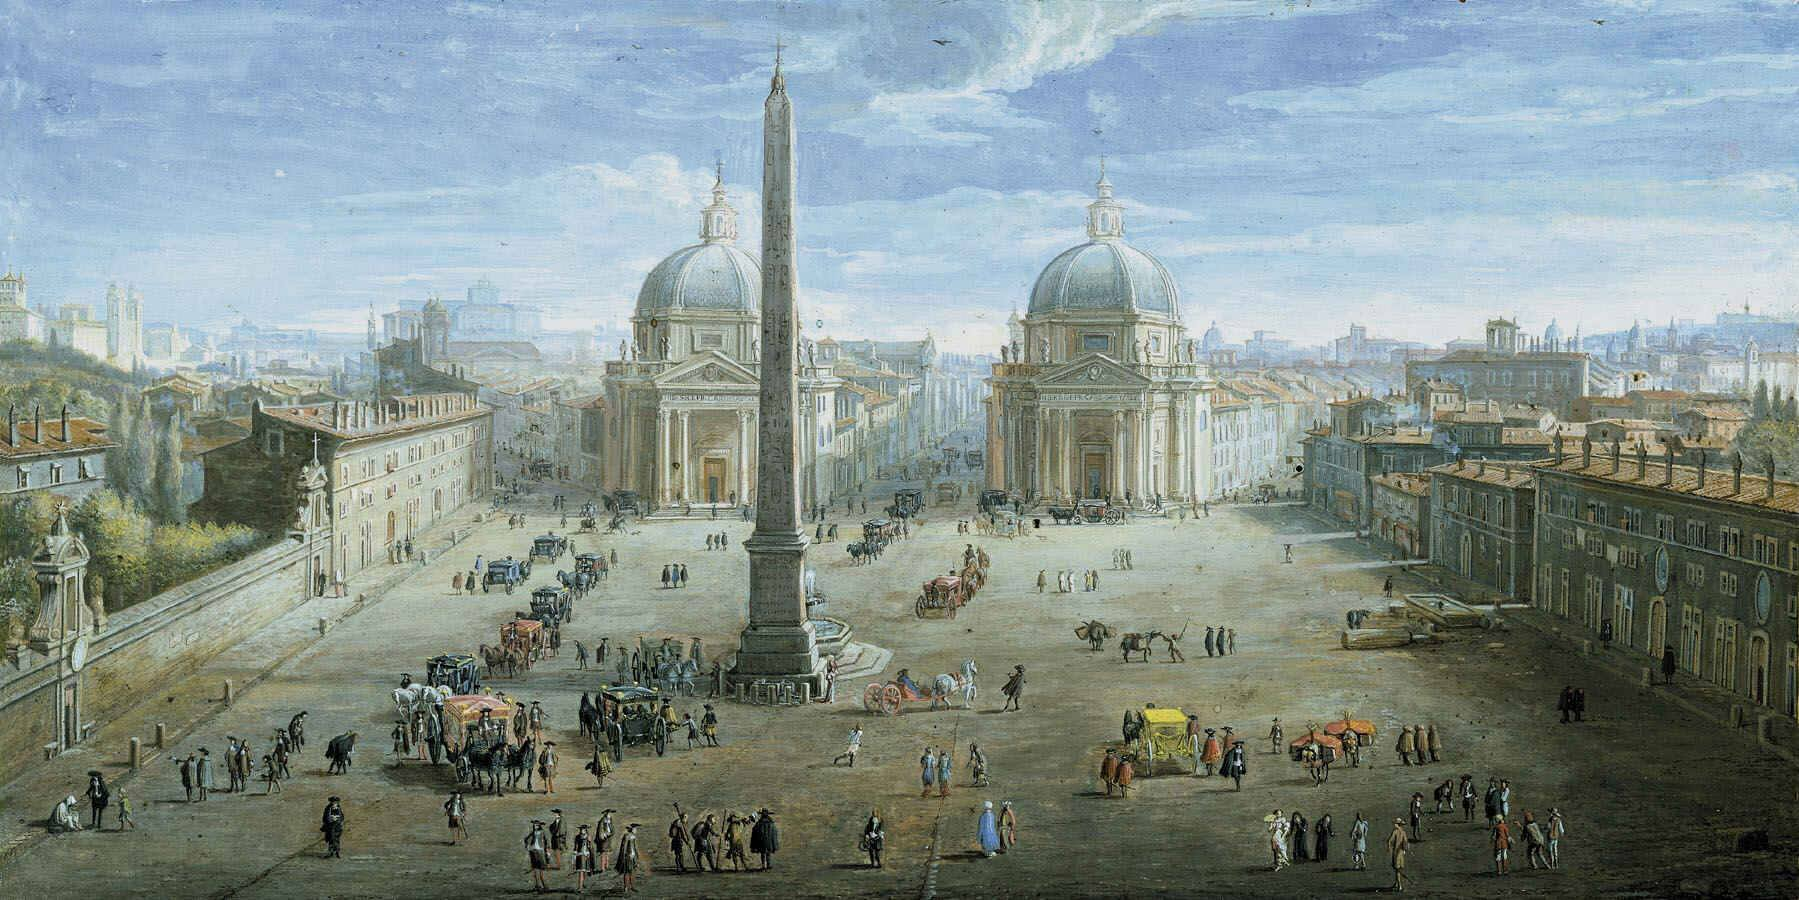
\includegraphics[width=1\textwidth]{/Users/Pancratii/GitHub/phd/Sections/Projeto_de_Pesquisa_2023-03-18_Teste/Pictures/popolo.jpeg} 
	\captionsetup{labelfont=bf}
	\caption{Vista da \textit{Piazza del Popolo}, em Roma, por Caspar Van Wittel (1652–1736). \textbf{Fonte:} Wikimedia Commons / Sotherby`s (coleção privada).}
	\label{fig:popolo}
\end{figure}   

Discorramos rapidamente sobre a ideia de \textit{forma} e traçado. Traçado é o particípio do verbo traçar, \textit{i.e.,} desenhar traços, riscar, sendo o ato ou efeito desse mesmo verbo, resultando, portando, em um `conjunto de traços', ou, no nosso caso, no `desenho que representa uma estrutura arquitetônica ou urbanística', o que é equivalente a dizer `planta', `projeto', ou, para usar um termo mais antigo, `traça' (PRIBERAM, TRAÇADO, 2023). Na língua rústica do latim, `tracto' que dizer `traçar sulcos', e `tractus' é a `delimitação por meio de traços; região, lugar, quarteirão' (FARIA, 1962, p. 1010). Penso que não haja melhor definição que essa: `delimitação por meio de traços' – que corrobora com a ideia de trajetória de estrada ou mesmo linha férrea (PRIBERAM, TRAÇADO, 2023). \textit{Forma,} porém, é um termo mais complexo.

 \begin{figure}
	\centering
	\includegraphics[width=1\textwidth]{/Users/Pancratii/GitHub/phd/Sections/Projeto_de_Pesquisa_2023-03-18_Teste/Pictures/nolli_popolo.png}
	\captionsetup{labelfont=bf}
	\caption{\textit{La nuova topografia di Roma} (detalhe), de Gianbattista Nolli (1701-1756), com a \textit{Piazza del Popolo} ao norte. \textbf{Fonte:} UC Berkeley Library.}
	\label{fig:nolli_popolo}
\end{figure} 

\textit{Forma} é a `configuração das coisas na parte exterior', o que é equivalente a `feitio' e `formato' (PRIMERAM, FORMA, 2023). No latim, a coisa complica um pouco, com \textit{`forma'} querendo dizer `fôrma' (que em português é um `molde sobre o qual ou dentro do qual se coloca alguma substância fluida, que toma o feitio desse molde'), ou `todo objeto feito na fôrma'; pode, de fato, ser entendida como `desenho, modelo, planta', mas também pode ser entendida como `tipo ideal', ou ainda como `conformação, configuração, constituição' (FARIA, 1962, p. 407). E, se formos para o campo da filosofia, aí é que a confusão aumenta, pois temos um `sentido filosófico e particularmente metafísico', um `sentido lógico', outro `epistemológico', um metodológico', e, por fim, ainda um `sentido estético' (MORA, 2001b, p. 1126) – e, portanto, a ideia de \textit{`forma'} escapa-nos neste momento.

Desse modo, na presente pesquisa, meu foco se direciona ao `traçado urbano' e não à \textit{`forma} urbana'. No entanto, é necessário esclarecer que o termo `traçado urbano', por sua vez, pode ter mais de uma acepção. Se pensarmos que a \textit{`forma'} da cidade é constituída por seu aspecto tridimensional,\footnote[6]{Aqui faço minhas as palavras de José Lamas (2010, pp. 41 e 48), ao dizer que a forma urbana corresponde "ao meio urbano como arquitectura, ou seja, um conjunto de objectos arquitectónicos ligados entre si por relações espaciais" e que é "a materialização no espaço da resposta a um contexto preciso".} com suas edificações e demais estruturas, podemos deduzir que o `traçado' é a marca deixada no solo por essa \textit{`forma'}. Logo, o `traçado' da cidade seria o sulco resultante dos limites dos lotes e quarteirões e dos contornos edificados (que, não raro, definem o próprio desenho das vias, por meio da conjunção de fachadas).\footnote[7]{Note-se que, diferente do que atualmente é lugar comum, o que definia o que era ou não a rua, seu limite, seu contorno, seu espaço, era precisamente a fachada da edificação, que imprime essa linha ao mesmo tempo imaginária e real no solo, diferente do que ocorre hoje. Hoje, o lugar comum é aquele de que o que define a via é o meio-fio — ou o limite do lote, que não coincide com a implantação da edificação, com a marca que a mesma deixa sobre o solo. E isso é fruto da desvinculação entre edificação e lote, entre os limites da edificação e os limites do lote. Mas, se olharmos para nosso passado urbano, veremos algo bem diferente. Basta olharmos uma pintura de Caspar Van Wittel da \textit{Piazza Navona} em Roma e veremos como a praça já era muitíssimo bem definida (pelas edificações), mesmo sem qualquer indício de calçamento, e muito menos de meio-fio.} 

No entanto, aqui, pretendo que o termo `traçado urbano' tome uma ênfase particular. Isso não exclui o sentido aludido acima, posto que tratarei de contornos edificados, lotes e quarteirões ao falar de `traçado urbano' ao longo desta tese – porém serei específico quando o fizer. Desse modo, a ênfase que quero dar é a de `traçado urbano' enquanto sinônimo de `espaço público', tanto na definição de Vitor Oliveira (2016)\footnote[8]{\textit{`The public spaces system of a city includes (...) the open spaces for movement, which we designate, in a simplified way, as streets, (...) [and] also the open spaces for permanence, which we designate as squares and gardens.'} (OLIVEIRA, 2016, p. 17).} quanto, particularmente, na visão de Huimin Ji e Wowo Ding (2021) – que trazem uma releitura contemporânea de Gianbattista Nolli (Figura \ref{fig:nolli_popolo}). Assim, o termo `traçado urbano' se relaciona com as vias, praças e áreas públicas de edificações – espaços com acesso franqueado ao público. Percursos, nós e polos abertos e fechados, cobertos e descobertos, percorríveis em um único plano contínuo: o plano do solo.\footnote[9]{Podemos chamar esse plano de `térreo', ainda que ele comporte variações de altitude e inclinação; porém a ideia é a de que esse é o "plano-base" da cidade, a partir do qual se desenvolvem as edificações, para cima ou para baixo.} Por vias podemos tomar percursos como ruas, calçadões, \textit{woonerfs}, escadarias e alamedas e espaços abertos de parques urbanos (excluídos os maciços vegetais), levando em conta a apropriação dos elementos contidos nesses espaços, como ocorre com os canteiros (HANNES, 2016);\footnote[10]{Canteiros que, atualmente, são considerados algo à parte, algo que não é inerente à via, mas que a define e delimita, posto que, para boa parte das prefeituras, o que determina o limite da via não é o \textit{continuum} das fachadas das edificações, senão o limite dos lotes (muros), as guias de meio-fio e os canteiros: elementos definidores da rua que não mais estão destinados a um uso comum.} bem como estacionamentos descobertos, além de rodovias e ferrovias (posto que servem de passagem para pessoas e suas mercadorias e que possuem uma marca sobre o solo que se relaciona com o desenho do restante da cidade). Por praças, podemos entender tanto a clássica praça, espaço aberto de dimensões superiores à da rua, o largo, o \textit{pocket park}, desde que descobertos – exceção feita aos \textit{`annodamenti'} (dos quais se tratará no momento oportuno), que ficam em uma situação ambígua de área pública de edificação e praça. E as áreas públicas de edificações podem ser exemplificadas pelas naves das igrejas, pelas platéias dos teatros e pelos halls, corredores, pátios e praças cobertas dos  edifícios públicos, galerias comerciais, mercados e \textit{shopping centers}.

Dito isso, reforço que: em relação às `formas' edificadas, conhecemos os motivos da crise atual  – e podemos mesmo ir mais a fundo, entendendo as dinâmicas inerentes aos materiais, à economia, às tendências ditadas de tempos em tempos pelas publicações e sua relação com o design de outras áreas. Temos ideia de como estabelecer um liame com o passado, inclusive com exemplos projetuais – e, quando não (como no caso do Brasil), temos um método para `ler' as pré-existências edificadas e, a partir delas, deduzir o \textit{tipo} edilício de um território, de modo a ter o balizador para novas edificações. E nisso reside a força da escola italiana de tipomorfologia urbana. Todavia, mais uma vez: se podemos sabemos como obter respostas em relação à \textit{forma} da cidade, o mesmo não se dá em relação ao seu traçado.

\section{O que(?)}
%Um método de projetação de traçados urbanos

Feito o invitatório, faz-se necessário clarificar alguns pontos acerca da tese que ora escrevo. E penso que valha a pena começar tratando por aquilo que ela `não' é. Ela não é uma tese filosófica, que tratará acerca da beleza ou da feiúra das cidades. Tampouco falará de `harmonia' de maneira abstrata, algo como a \textit{Divina Proportione}. Ou de \textit{Simetria}, ou de simbolismo, ou mesmo de pinturicidade e legibilidade das cidades – muito embora meu trabalho termine por incidir tangencialmente sobre esses temas. Ao contrário, minha tese está mais para uma espécie de tratado. E isso mais porque pretendo desenvolver algo feito à mão e sobre algo muito cru, sem muitas abstrações. E não porque darei novas definições para o \textit{universo mundo} da arquitetura (no qual o desenho urbano se insere), posto que aqui pretendo desenvolver um método. Um método? Sim. Mas um método de quê? Um método de como projetar traçados urbanos, e disso trato a seguir.

\section{Por que(?)}
% Problematica


\textit{"We suggest that the time has come, in this ‘age of sustainability’, to mount a challenge to the very model of industrial design, and the sculptural fine art that has, however much it aspires to be more, served only as so much specialized ‘product packaging’. To that extent, it has only served to co-conspire in the damage done by this top-down regime. [We] must exploit these very same emergent and collaborative processes of adaptive morphogenesis – the ones that perform so well in natural systems."} (Mehaffy, 2011, p. 494).

\section{Como(?)}
%Método científico, protocolos, etapas.

\section{Quanto(?)}
%cronogramas (etapa concernente ao projeto de pesquisa)

%28ABR2023 08:55 Aula Codinhoto
	%Minha pesquisa é indutiva, não? Pega indícios (segundo o que tenho visto das aulas do prof. Codinhoto))


	\chapter{Conceituação}

			\section{Revisão Bibliográfica}

			É necessário estabelecer aqui uma coisa. O artefato que pretendo ter desenvolvido ao fim desta tese é um `conjunto de diretrizes' voltado ao ato, ao processo de projetar traçados urbanos. Seu intuito será, portanto, nortear cada uma das decisões tomadas durante esse processo, a depender das variáveis e circunstâncias que se apresentem ao projetista, pesquisador, professor ou aluno. Dito isso, vale lembrar que os artefatos que mais se aproximam da ideia de `conjunto de diretrizes' não estão em artigos científicos, mas sim em guias, manuais, ou mesmo cartilhas – algo muito mais prático, \textit{i. e.,} mais à mão do usuário final, ainda que solidamente baseados nos conceitos e métodos divulgados pelos artigos científicos. Desse modo, terei duas revisões de literatura. Uma revisão assistemática, de maneira a formular um \textit{core} sistematizado de conceitos (constructos). E uma revisão sistemática de literatura com vistas a identificar artefatos semelhantes ao que pretendo desenvolver.

				\subsection{Revisão Assistemática de Literatura (RAL): \textit{il `core' della ricerca}}

				Escola italiana de tipomorfologia

				\subsection{Revisão Sistemática de Literatura (RSL/RBS): \textit{l`artefatto}}
				Entendido o \textit{core} de autores seminais e o \textit{framework} teórico-metodológico e projetual com o qual estou a trabalhar, parto para uma Revisão Sistemática de Literatura (RSL) – ou Revisão de Bibliografia Sistemática (RBS). Nela, sigo os passos descritos por Dresch, Lacerda e Antunes Jr. (2015).

				Como meu artefato é um `conjunto de diretrizes' voltado ao ato, ao processo de projetar traçados urbanos, aquilo que posso encontrar de mais próximo dele são os \textit{`design guidelines'}, comuns ao universo anglo-saxão – mas que não necessariamente tratam de fatores ligados ao \textit{rendimento}: é por essa razão que a presente revisão sistemática de literatura foca sobre eles por meio do protocolo a seguir.

					\textbf{Protocolo para revisão sistemática}

					\textbf{Framework conceitual:} \textit{rendimento} (Caniggia, 1963; Caniggia e Maffei, 2008; Carlotti, 1995, 2012; Cataldi, 2003; Dalla Negra, 2015; De Martin, 2009; Marzot, 2015; Maffei, 2003; Rebecchini, 2008), \textit{rendimento} urbano (Costa, 2020; Costa e Rego, 2019).

					\textbf{Contexto:} Novos traçados urbanos.

					\textbf{Horizonte (a):} Traçados \textit{ex novo}: 
					\begin{enumerate}
						\item (a) apenas sobre relevo, 
						\item (b) sobre parcelamentos rurais precedentes, \item (c) sobre outras estruturas antrópicas (diretrizes viárias, faixas de domínio).
					\end{enumerate}

					\textbf{Horizonte (b):} 
					\begin{enumerate}
						\item Áreas não urbanizadas (expansão urbana \textit{in nuce}), 
						\item franjas peri-urbanas (expansão urbana \textit{in fieri}), 
						\item vazios urbanos (dita `especulação').
					\end{enumerate}

					\textbf{Corrente teórica:} `Cidade como organismo' – escola italiana de tipomorfologia urbana.

					\textbf{Questão de revisão:} O que existe, dentro do universo dos guias e/ou manuais com diretrizes/instruções de desenho/parcelamento urbano (\textit{urban design guidelines, guides/manuals}), que contemple, ou pelo menos se aproxime, na teoria e/ou na prática, do arcabouço teórico-metodológico da escola italiana de tipomorfologia, ou ao menos do conceito de \textit{rendimento} urbano?

					\textbf{Estratégia de revisão:} Agregativa ou Configurativa?

					\textbf{Critérios de busca:} \textbf{(a)} Critérios de inclusão (tratar diretamente de questões relacionadas ao \textit{rendimento} urbano); \textbf{(b)} Critérios de exclusão: (máximo 10 manuais/guias, 10 artigos, 5 livros) 1. Ordem de exposição na busca (relevância?), 2. Título (se tem a ver ou não com a tese), 3. Abstract, 4. Sumário, 5. Conteúdo \textit{in se} (a. imagens [grafos, mapas e projetos] do processo de formação de traçados ou de traçados prontos, b. texto).

					\textbf{Termos de busca:} design guidelines for residential areas (Milena), design guides (Renato), urban design guides/manuals, slope, walkability + slope, urban design, urban layouts, urban methods, design guidelines, morphogenesis, urban design guides, waldhufendorf, urban design guidelines, urban design manuals.

					\textbf{Fontes de busca:} Google Acadêmico, Scopus|Elsevier, Scielo, Revistas (U+D Urbanform and Design [italiano], Urban Morphology [inglês], Revista de Morfologia Urbana [português], Nature [inglês], Planning Perspectives [inglês]).

					Indicadores Boleanos: "AND" e "OR"

					Termos: "Urban", "Design", "Layout", "Guidelines", "Manual".
					Tentativa 1: Periódicos Capes 02SET2023 22:00 Urban E Design E Guideline*


					Tentativa 2: Periódicos Capes 02SET2023 22:04: Urban E Design E Guideline* E Layout E slope
					Resultado: Moser, W. A. (1991). Design for Successful Hillside Development. Journal of Urban Planning and Development, 117(3), 85–94.

					Termos: "Urban", "Design", "Layout", "Guidelines", "Manual", "Standards", "Slope", "Walkability", "Sustainability".

					`Urban' AND `Design' AND `Layout' AND `Guidelines' AND `Slope' AND `Walkability' and `Sustainability'

				


			\sout{exemplo}
	\section{Estado da Arte}
	\section{Referencial Teórico}
	\section{Sustentabilidade}
%24ABR2023 21:11
%Livro Maretto WAM (descrição correta de unidades de vizinhança, polaridades, sustentabilidade, etc.), link morfologia e sustentabilidade
	%https://books.google.com.br/books?id=t_TDCQAAQBAJ&printsec=frontcover&hl=pt-BR#v=onepage&q&f=false
	%https://books.google.com.br/books?id=Y_ugDgAAQBAJ&printsec=frontcover&hl=pt-BR#v=onepage&q&f=false
% Artigo Maretto sobre Muratori: link entre MURATORI e a ESCOLA ITALIANA com a SUSTENTABILIDADE (não só ambiental, mas projetual como um todo: ambiental, social, econômica, etc.)

%25ABR2023 01:02 Procurando uma ligação entre Unwin e a escola italiana de morfologia urbana, deparei-me com um link na obra de Saverio Muratori, sobretudo em seus projetos urbanos. A saber: por mais que não bebam da mesma fonte Unwin e Muratori se assemelham por suas diretrizes projetuais, sobretudo se observadas à luz dos atuais princípios de sustentabilidade e de exemplos projetuais que se concretizaram "successfully", como Slusehølmen, Skarvet, Expo 98, Quartiere Quinto, entre outros.

\section{Morfologia urbana}
%24ABR2023 21:09
%Artigo Maretto (corrigir artigo na tese, com base no livro)
	%Anotação para Renato: "Estou com muitas coisas na cabeça depois de reler esse artigo.
		%1. Realmente Muratori estava à frente do seu tempo (veja-se a questão de serviços públicos como até centros para idosos em unidades de vizinhança e o aspecto da sustentabilidade, com a vinculação dos terraceamentos, topografia e arborização);
		%2. Só agora me dei conta de que o projeto dos estuários I e II são praticamente o que temos hoje no Slusehølmen em Copenhagen,  e na Expo 98 de Lisboa;
		%3 e mais importante: é IMPRESSIONANTE a semelhança do raciocínio dele com os princípios de Unwin!
		%Renato, você é um gênio! Finalmente achei um link que una ambos! Obrigado."

%Fica apenas um gap por hora: os bairros de Muratori eram restritos, enquanto eu estou pensando numa \textit{urbs}, numa cidade que se expande, numa metrópole, pois é a escala que teremos doravante (ou ao menos de algo que sirva do pequeno assentamento à metrópole a partir da morfologia do sítio).

%25ABR2023 01:50 Há uma questão de escala aqui. Uma cidade Muratoriana (como as Barene di San Giuliano) muitas vezes, para nós, não passam mais do que bairros. A cidade é muito maior.

%01MAI2023 11:28
	%Se observarmos os projetos de Unwin para Letchworth e Hampstead, veremos pouca ou menor consideração pelo relevo do que por um traçado curvilíneo olhado desde cima – o que pode gerar perspectivas, mas que não é necessariamente vinculado à topografia e a todas as suas variáveis e consequências (como caminhabilidade, etc.). Já Muratori leva a morfologia do sítio com afinco em seus projetos, ainda que estes apresentem, diferente de Unwin, conjuntos edificados retilíneos (ao invés de lotes em vias curvas). Não chegam a ser tese e antítese, mas são dissonâncias que podem ser harmonizadas. Logo, o ponto será fazer lotes em vias curvas geradas a partir da topografia (bem como tratar dos edifícios vinculados a ela – ao menos os principais edifícios).
	
	\subsection{Espaço público e privado}
	%18JUN2023 05:29
	Quando falo em `espaço público' (open space), estou me referindo ao espaço público, semi-público ou privativo com acesso ao público, de ruas e praças ao interior de igrejas. teatros e shoppings centers. Seriam uma espécie de "vão servente" da cidade (se fizermos o paralelo com a classificação entre vãos serventes e servidos própria da escola italiana de tipomorfologia). Já o `espaço privado' é o equivalente ao "vão servido", ou seja, o vão que só pode ser acessado por meio de um vão servente: do interior das lojas e supermercados ao interior das casas. Meu entendendimento, portanto, não parte de um ponto jurídico e positivista do que é o espaço público ou privado – ou seja, de `propriedade' pública ou privada segundo tal ou qual lei presentemente em voga. Ao contrário, minha acepção parte de um ponto de vista morfológico, relacionado à possibilidade real de acesso/ingresso a esse espaço, que redunda na sua morfologia, em sua forma, em sua abertura para espaços cada vez mais amplos e acessíveis (topologicamente falando). Exemplo? A nave de uma igreja que se abre para a rua; a praça de alimentação de um shopping center que se conecta a `ruas' internas à edificação (corredores), chegando finalmente à rua externa; o pátio ou \textit{hall} de um paço público. Todos esses são extensões do espaço público. Espaços públicos (abertos ou cobertos) cujo acesso é franqueado indiscriminadamente à população (mesmo considerando possíveis distorções como a acepção de pessoas em determinados ambientes e horários, posto que, em princípio, o espaço é feito para ser acessado por todos – tanto os que precisam do aspecto apologético da igreja, tanto quanto os que precisam do `capitalismo' consumista do \textit{shopping center}).
	
	\textit{Open Spaces} (PATTACINI, 2021)
	
\section{Estruturas naturais: cumeadas, talvegues, linhas de encosta (ou meia pendência)}

Acerca das estruturas naturais do território, em termos de nomenclatura, penso que me posso continuar fiando da dissertação de Maria Rosália Guerreiro (2002). Em seu segundo capítulo, "[a] estrutura natural do território", em particular, há referências a obras que tratam da definição dos pormenores do relevo. Obras às quais infelizmente não obtive acesso direto – motivo pelo qual tal dissertação merece crédito, ao trazer extensas citações diretas e imagens, assegurando a checagem de dados.

Um `centro de distribuição' ou um `centro de encontro' (Guerreiro, 2002, p. 53) podem ser polos em potencial. Mas, afinal, o que define um `polo em potencial'? Sabemos que um nó é um ponto de cruzamento de dois contínuos de mesma natureza (como dois percursos), ou de atravessamento de um contínuo sobre outro contínuo de natureza distinta (um percurso sobre um rio). E, se olharmos do ponto de vista dos grafos, um `nó' seria o ponto de encontro de três ou quatro grafos, especificamente. Dois não poderiam ser, pois isso, por exemplo, seria apenas um ponto de inflexão em um percurso. Três, porém, podem representar duas seções de um percurso intersectadas por outro, ou um percurso que para às margens de um rio. Quatro grafos, por sua vez, seriam as seções de dois percursos ou de um rio e um percurso. No entanto, cinco grafos já mostrariam uma condição de derivação ou confluência para aquele ponto – fator que mais caracterizaria um polo que um nó.

Se pensarmos sob a lógica dos centros de distribuição e encontro, apenas, encontraremos uma contradição ao perceber que Roma, por exemplo, não foi fundada na confluência de afluentes do Rio Tibre, ou em um ponto de confluência de cumeadas sobre um único maciço. Muito pelo contrário. Reforço, o que ocorreu foi exatamente o oposto. Foram terminações de cumeadas (as sete colinas, que davam origem – ou fim – àqueles caminhos que levam à Cidade Eterna) que confluíram em uma área plana do Tibre. Cada margem do rio era o limite intransponível de uma civilização, até que os limites foram superados com o atravessamento da Ilha Tiberina (Caniggia e Maffei, 2008). Logo, o critério para a constituição de um polo urbano é mais complexo do que apenas a convergência hierárquica das cumeadas ou talvegues à guisa de 'árvore'. E, nesse sentido, o que se deve levar em conta é a convergência dessas estruturas, porém, de maneira mais complexa e variável, a depender das características do local.

\section{Estruturas antrópicas: percursos, nós, polos e tecidos}
%18JUN2023 04:07 Faz mais de uma ou duas semanas que estou enrolado com esses conceitos, sobretudo com a distinção entre nós, nodalidades, polos e polaridades, que parece ser ambígua entre open spaces e edilícia. Ontem discutíamos eu, Luiz e Luca sobre isso e fiz diversas anotações pertinentes no caderno, chegando ao método. O método tenho já relativamente delineado (ao menos em princípio). Falta lapidar esses conceitos e o próprio método em si.) 
	%Para as estruturas naturais, recordo da Maria Rosália Guerreiro – e penso que a Teresa Marat-Mendes tenha algo, assim como o Ian McHarg, não? Isso sem falar nos próprios Caniggia e Maffei e Carlotti (mas, no caso desses três últimos, penso que a coisa se refira mais a __como__ aproveitar essas estruturas naturais).
	% Já para as estruturas antrópicas, não posso senão falar exaustivamente de Caniggia e Maffei, Carlotti e Maretto (e mesmo do artigo que traduzi com o Renato).
%18JUN2023 04:31 Observando o mapa do território de São Paulo e do Paraná com as cumeadas, bacias e ferrovia Sorocabana (que desenvolvi na dissertação, p. 59), é interessante notar que o rio Paraná será um polo final para a cumeada que atravessa o território da CTNP (faltando apenas definir onde seria o polo inicial); para a ferrovia, poderíamos adotar a travessia do rio Tibagi como primeiro nó, terminando no rio Ivaí (ou talvez em Cianorte); porém, se observarmos a conjunção dos dois fatores e a estruturação (parcelamento) do território, podemos – realmente – pensar em Londrina e Maringá como duas polaridades territoriais, posto que é nesses dois polos (nessas duas cidades) que ocorre uma "inflexão", uma mudança: a saber, a ferrovia deixa de subir o relevo para passar a se assentar sobre o traçado da cumeada territorial, dando origem a um território único (unitário).

	\chapter{Um novo estudo de caso sobre Maringá}
	\section{Uma análise de Unwin}

	Iniciemos pelo sumário da obra de Raymond Unwin. Após o prefácio temos os seguintes capítulos:
	\begin{enumerate}
		\item \textit{Of Civic Art as the Expression of Civic Life};
		\item \textit{Of the Individuality of Towns, with a Slight Sketch of the Ancient Art of Town Planning};
		\item \textit{Of Formal and Informal Beauty};
		\item \textit{Of the City Survey};
		\item \textit{Of Boundaries and Approaches};
		\item \textit{Of Centres and Enclosed Places};
		\item \textit{Of the Arrangement of Main Roads, their Treatment and Planting};
		\item \textit{Of Site Planning and Residential Roads};
		\item \textit{Of Plots and the Spacing and Placing of Buildings and Fences};
		\item \textit{Of Buildings, and how the variety of Each must be dominated by the Harmony of the Whole};
		\item \textit{Of Co-operation in Site Planning, and how Common Enjoyment benefits the Individual};
		\item \textit{Of Building Bye-laws}.
	\end{enumerate}
	
	\chapter{\textit{Modus faciendi} atual (entrevistas)}
%10JUN2023 17:52 CASA
%Em que vamos agir, incidir, senão sobre o \textit{modus faciendi} atual? (Isso faz da minha pesquisa uma DSR, na qual busco incrementar ou aperfeiçoar um método existente? Ou não?). Ora, e o que é esse modus faciendi atual? Ou melhor, como se projetam loteamentos e novas áreas urbanas atualmente? Onde posso descobrir isso? – Mascaró e outros autores podem me ajudar. A grande questão é descobrir de onde Mascaró tirou suas fontes (a não se que seja tudo empírico) e que livros, no Brasil e no exterior, ensinam como projetar traçados urbanos, de modo a entender sua lógica e como ela pode ser `capovolta'.)

	\	chapter{Variações sobre um tema: o processo de projeto de um novo traçado urbano em diversos cenários}

Como costumo trabalhar ouvindo música, é natural que termine por projetar seguindo um pouco da lógica dos compositores que ouço, ou ao menos da estrutura impressa em suas composições. %(da lógica impressa na estrutura de suas composições).
Logo, não me posso furtar da analogia entre arquitetura e música. Não daquela analogia entre proporções, como existe entre ordens arquitetônicas, escala musical e proporções matemáticas – essa deixo para aqueles que são mais pitagóricos, mais platônicos do que eu; ou ao menos para aqueles mais versados nesse tema. Ao contrário, minha analogia se dá na estruturação, da lógica compositiva. A analogia entre o processo de projeto e o processo de composição, entre o traçado e sua configuração impressa no solo e a estrutura musical (nas formas em que veremos a seguir, como variações sobre um tema, forma cíclica, etc.).

Aqui, as estruturas naturais serão meu "tema" e o traçado urbano o ulterior "desenvolvimento" desse "tema".

%27ABR2023 14:17 Ainda sobre o artigo do Maretto sobre Muratori.
	%Note-se que Muratori projetava com percursos principais, secundários, unidades de vizinhança, edificações baseadas no tipo, etc. Ora, diante disso, que contribuição inovadora eu posso dar? O método já está todo ali. Bom, algo está ligado à questão de escala. Muratori fazia apenas pequenas cidades (que até poderiam se expandir, mas que eram estanques em si mesmas enquanto projetos), enquanto hoje temos metrópoles, que seriam (em termos de escala) iguais a uma somatória de diversas dessas cidades, o que me faz pensar em projetar conforme Muratori, mas sempre pensando no meu framework de maior escala de modo a formar um grande quadro urbano a partir de pequenas cidades muratorianas (o que, para mim, ou para o próprio Unwin e Vieira, seriam bairros) – há que se ver o que Muratori entende como "cidade" (é apenas morfológico? Depende de quais polaridades? Quais equipamentos?). Além disso, há uma outra questão, não apenas de escala, mas de logística e temporalidade, i. e., Muratori projetava os edifícios prontos – o que é diferente da nossa realidade – e cidades que eram pequenas (pequenas unidades, como já mencionei), porém, como são as unidades de terra, os lotes? Cada quadra seria já um lote? Isso funciona talvez numa Expo `98, mas será se funciona no Brasil. Posso abrir os percursos conforme o relevo e fazer um Skarvet da vida, com uma quadra-lote, ou talvez um Slusehølmen da vida, com um grande quarteirão que deixa um espaço aberto interno (enquanto os apartamentos constituiríam os lotes). Talvez. Mas isso é possível? É factível? Sim e sim. Mas é viável? Isso já não sei (e que o diga Goiânia). Isso sem mencionar que a nossa lógica é aquela lógica lusa em que temos ruas com lotes e quintais e que nossas unidades de vizinhança (muratorianas) se dão mais pela praça pública do que por uma espécie de praça semi-pública (como no mundo anglo-saxão) – embora tivéssemos os cortiços e paços. Desse modo, preciso pensar em projetar numa escala maior que a cidade muratoriana e de tal modo que o traçado incorpore os lotes de modo a direcionar, talvez, o formato dos edifícios, mas sem necessariamente os determinar (como o faria Muratori), de modo a tornar viável em escala, espaço, logística e tempo.
		%% 27ABR2023 15:18 No caso da escala e dos projetos de pequenas cidades integradas entre si formando um conjunto, isso poderia entrar como cunhas verdes, cidades-satélites, cidade-região ou algo assim?

	\chapter{Método}
\section{Passo-a-passo}

\part[Desenvolvimento]{Desenvolvimento}
	
	\chapter{Protocolo (desenvolvimento do artefato)}
	\chapter{Diretrizes projetuais}
	
	%2023-09-15 20:58 CASA – método/diretriz de projeto
	Algo que pode ser feito é: ao invés de projetar e implementar o loteamento de uma vez, é projetar o loteamento (com base nas linhas do relevo e na hierarquização dos percursos), mas só implementar aos poucos. Ou seja, no percurso territorial apoiam-se diversos lotes, distribuídos em faixas – e essas faixas podem ser parte de quarteirões que seguem o sentido do percurso territorial. Assim, o percurso territorial se torna um percurso matriz. Após a venda desses lotes (ou de um percentual significativo deles – seja do percentual da faixa inteira, ou dos quarteirões individuais), pode-se criar uma nova faixa de lotes paralela à primeira e aí vender os lotes. E assim sucessivamente. E, entre uma fase de vendas e outra, pode-se fazer uma análise com a metodologia \textit{Morpho}, e fazer eventuais alterações no projeto do loteamento, o que pode garantir maior diversidade de formas, diferente de um projeto concebido e executado todo em uma única tacada, e talvez apenas por um único profissional. Além disso, vale observar quais usos foram implementados nos lotes, a fim de gerar uma base de dados da qual se possa extrair a relação de uso dos lotes por percurso e fase de execução do loteamento e crescimento da cidade.

	Outra coisa. Eu sempre dizia que as áreas que serão áreas verdes dentro das áreas urbanas devem ser separadas \textit{a priori} pelo governo ou ente responsável pelo gerenciamento da urbanização (como o foi a Companhia em Maringá, por exemplo). Agora eu vou além: não é apenas delimitar e remover os fundos de vale antes da venda dos lotes rurais, ou comprá-los antes da urbanização da área, antes, é necessário fazer um projeto paisagístico, de modo a dar uma função antrópica `com propósito', que faça sentido para o indivíduo comum, que não apenas a mera preservação, que faz apenas `delimitar' a área com uma violenta barreira (como o são os gradis, não pelo material com que são feitos, mas por não haver gradação na transição entre área acessível e área restrita). Parques, bosques, tudo isso deve servir como um grande \textit{framework} que `precede' – \textit{nota bene}, `precede' – a urbanização.

\part[Avaliação]{Avaliação}
	\chapter{Comparativo com o existente (estudo de caso)}
	\chapter{Grupos focais e \textit{feedback}}
	\chapter{Diretrizes projetuais (artefato – versão refinada)}

\chapter*{Referências}
\addcontentsline{toc}{chapter}{Referências}	

\chapter*{Anexos}
\addcontentsline{toc}{chapter}{Anexos}

\section*{Descrição dos procedimentos efetuados, algoritmos e códigos}
%\addcontentsline{toc}{section}{Descrição dos procedimentos efetuados, algoritmos e códigos}


\end{document}          
